
\section{Introduction}
\label{sec:introduction}

The growth of the Linked Open Data (LOD)
cloud\footnote{\url{http://lod-cloud.net/}}
goes hand in hand with an increasing amount of geospatial information being made available
for online querying via SPARQL.
For instance, the community projects DBpedia and LinkedGeoData provide access
to more than 1.3 million and 2 billion point geometries based on Wikipedia and
OpenStreetMap data, respectively. Government agencies have started maintaining
public SPARQL endpoints, such as \emph{Ordnance
Survey}\footnote{\url{http://data.ordnancesurvey.co.uk}}
and the \emph{European Environment
Agency}\footnote{\url{http://semantic.eea.europa.eu/sparql}}.
The latter, for instance, hosts
% 9.321 RDF graphs, of which
123 RDF graphs that contain a sizable number of resources described using
the WGS84 vocabulary\footnote{\url{http://www.w3.org/2003/01/geo/wgs84_pos}}.
%instances.

%\footnote{\url{http://data.ordnancesurvey.co.uk/datasets/os-linked-data/explorer/sparql}}
% \footnote{\url{http://semantic.eea.europa.eu/sparql}}.
%The importance of geospatial data has also been recognized by many RDF store
%implementors, who over the past few years added and enhanced spatial support in
%their products.
Yet, the user friendly exploration of spatial data accessible via public SPARQL remains a
major challenge, especially due to performance, volume, scalability and UI
complexity issues.
In this demo, we present the spatial data exploration and
visualization application \emph{Facete}, depicted in
\autoref{fig:facete-screenshot}.
%\todo{Mention that Jassa makes these re-usable}
Facete is a client-side JavaScript application, which interacts with a server-side SPARQL endpoint.
The major problem when exploring spatial data is that the spatial dimension is in most cases not directly attached to all the data items.
For example, a dataset about multi-partner research projects would contain entities for the projects itself, the project partners, their legal entities, the branch offices of these legal entities and finally the cities they are located in.
If we want to visualize such data intuitively, we need to determine the path from data items of interest to the indirectly related spatial entities.
Facete solves this problem with a automatic discovery of the most likely property path.
Compared to other faceted browsers, Facete not only allows to constrain over facets of a particular set of entities, but over facets across full property paths.
This allows to explore data more intuitively and in ways previously impossible.

In the remainder, we explain Facete's user
interface in \autoref{sec:facete},
followed by a description of a use case
scenario in \autoref{sec:use-case}.
In \autoref{sec:concepts} we briefly outline the conceptual background of Facete's main components. Subsequently,
\autoref{sec:related-work} discusses related work. Finally,
\autoref{sec:conclusions} concludes and gives pointers to
future work.
Comprehensive accompanying material including the open-source code, screencasts and documentation can be found at \url{http://facete.aksw.org}.
%It is noteworthy, that Facete as described in this submission is an application.
%Application code itself is not aimed at reusability, in contrast to library code.
Under the umbrella of the
\emph{JAvascript Suite for Sparql Access
(Jassa)}\footnote{\url{https://github.com/GeoKnow/Jassa}} project, we are
working on making Facete's core components available as reusable library components,
which developers may reuse and customize as needed.


%The European Environment Agency maintains a SPARQL
%endpoint\footnote{\url{http://semantic.eea.europa.eu/sparql}} has started
%% publishing RDF, of which \todo{number} use the wgs84 vocabulary.
%9.321 named graphs having at least a single instance described using the WGS84
%geo positioning
%vocabulary\footnote{\url{http://www.w3.org/2003/01/geo/wgs84_pos}}.
%Among those graphs there are 123 graphs having more than 50 of such
%instances.


%%\todo{Mention deployment}
%%TODOyay\footnote{\url{http://open-data.europa.eu/semmap/}}

\section{The Facete SPARQL Explorer}
\label{sec:facete}
Facete is a Single Page Application (SPA) whose user interface comprises several
UI components, which are depicted in~\autoref{fig:facete-screenshot} and
explained in the following.
In the top area, there are elements that enable the user
to select a SPARQL endpoint and chose from one or more of its contained named graphs.
The main panel is divided into three columns containing a set of widgets with
the following functionality:
%\todo{Motivate that faceted search is superior (to what?) because one cannot
%hit dead ends} \todo{In conclusion, mention how the faceted search can also be
%% applied to statistical data, i.e. it is possible to create a datacube closure
%over ANY set of RDF resources; the facet module already does filtering by an
%arbitrary number of correlated dimensions.}
\emph{1. Selection.}
The first widget, labeled \emph{Facet}, shows a
  facet tree that corresponds to the properties of all resources that match the
  set constraint.
  If there are no constraints, all resources that appear as a subject in the
  selected graphs are matched.
  Three actions can be performed for node in the facet tree:
  A click on the facet's name lists the facet's values in the
  \emph{Facet Value} widget, where these values can be used for defining
  constraints. Clicking the caret symbol toggles the display of
  corresponding child facets. These are the properties of the the selected facet's values.
  Lastly, a facet can be pinned as a column to the \emph{Table View}.
  Note, that the root of the facet tree is formed by a facet labelled
  \emph{Item}. This facet's values correspond to the set of resources in
  subject positions of the selected RDF graphs.
The \emph{Facet Values} widget enables a user to paginate
  through a selected facet's values and optionally filter these values by a
  search term. Furthermore, clicking the checkbox next to a value creates a
  constraint.
The \emph{Filters} widget lists all active constraints.
  Individual constraints can be removed by clicking their entry, whereas the  
  \emph{Clear Filters} button purges them all. 


\emph{2. Data.}
The middle area contains the \emph{Table View}, which
  lists a table whose content is based on resources that match the active constraints
  and the facets that were pinned as columns.
  Columns can be sorted by clicking the caret icons. Multiple orders are
  supported by holding the shift key down while clicking.

\emph{3. Geographical.}
The \emph{Geo-Link} drop down menu enables the user to choose from
  property paths connecting the resources that match the constraints with those
  that can be shown on the map. By default, the option \emph{automatic} is
  enabled, which always picks the shortest path among the found ones.
The \emph{Map} widget displays markers corresponding to the
  selected resources and the geo-link. Blue boxes indicate areas that contain
  too many markers to be shown at once. These boxes disappear when
  sufficiently zoomed in. Clicking a marker shows its details in the
  \emph{Detail View}.
The \emph{Detail View} shows the excerpt of the \emph{Table View} that
  corresponds to the selected marker(s).

\begin{figure*}[t]
\centering
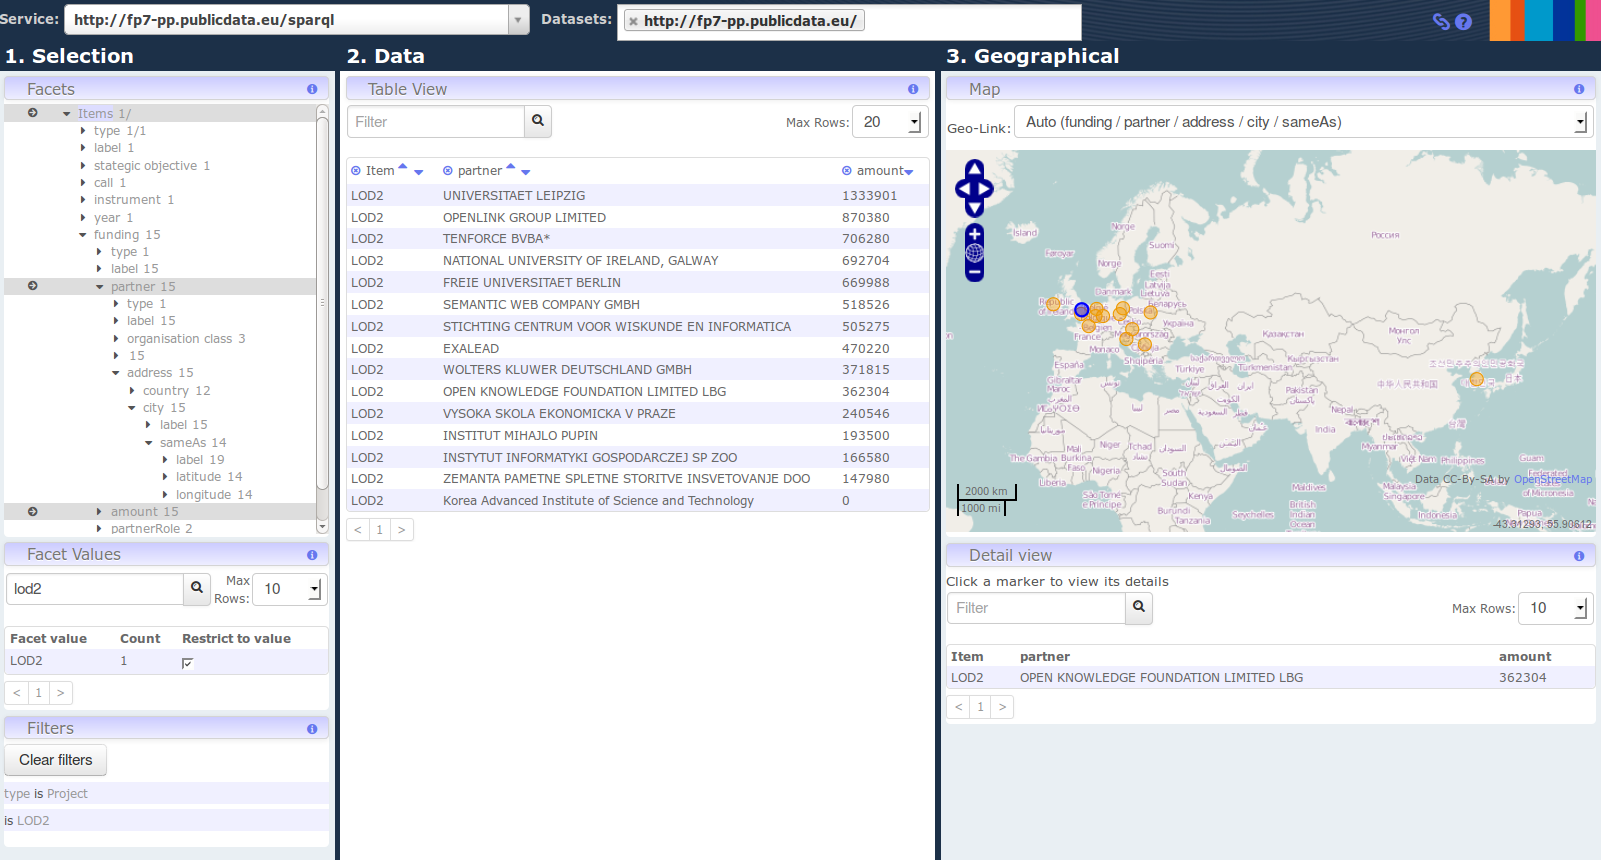
\includegraphics[width=\textwidth]{images/2013-12-19-odp-facete-2.png}
\caption{Screenshot of Facete showing information from the CORDIS dataset about FP7 research funding.}
\label{fig:facete-screenshot}
\end{figure*}


\section{A sophisticated Use Case}
\label{sec:use-case}
We demonstrate Facete in a use case scenario, which
to the best of our knowledge, none of the existing SPARQL browsers can serve
easily.

The dataset about \emph{ICT research projects under EU-FP7} 
\footnote{\url{http://open-data.europa.eu/en/data/dataset/ict-research-projects-under-eu-fp7}},
for which an RDF version
exists\footnote{\url{http://fp7-pp.publicdata.eu}}, 
contains comprehensive information about funded projects, partner organizations and particularly also how much money was granted to partners in FP7-ICT
projects.
The most important classes and their relations are as follows:
Every \emph{Project} is related to a set of \emph{Fundings} (grants), whereas each
instance represents the amount of money granted to a single project
partner (beneficiary). %Partners who received  (\todo{beneficiary}).
%Each funding targets a beneficiary, whereas beneficiaries may receive multiple
%fundings.
Partners carry address information, which includes resources for
the country and city. The cities' geo-coordinates were
obtained based on interlinking them with
\emph{LinkedGeoData}\footnote{\url{http://linkedgeodata.org}}.
This model is depicted in~\autoref{fig:relation-example}.
\begin{figure}
\centering
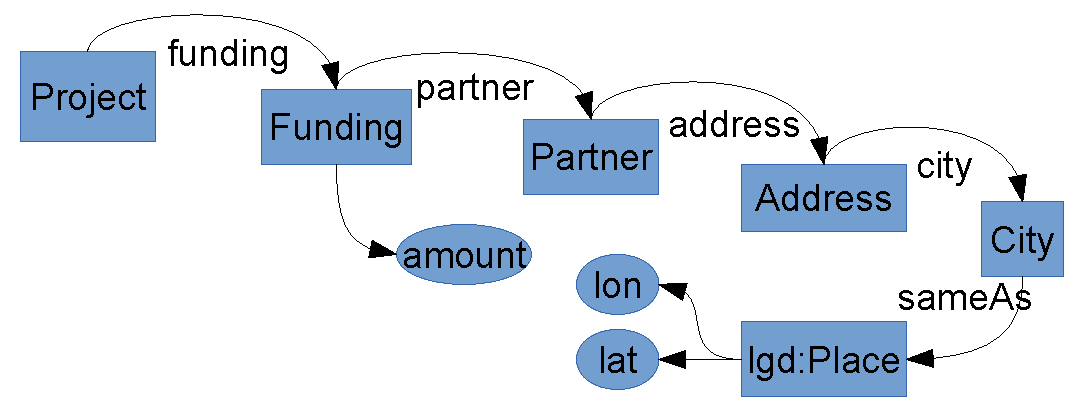
\includegraphics[width=0.5\textwidth]{images/RelationExample}
\caption{Excerpt of the CORDIS dataset model showing the path how projects are related to geo-coordinates.}
\label{fig:relation-example}
\end{figure}

There are several questions one may ask, such as:
What are the projects related to a certain country? 
Where are the partners of a particular project located?
How much money was granted to partners in a specific project?

With Facete, the following procedure can be performed to answer these questions:
\begin{itemize}
  \item First, select the \emph{type} facet, and constrain it to the value
  \emph{Project}. The main table will now only list project names, and the map
  component will automatically determine connections that link projects
  to coordinates.
  \item A project is related to a country if there is at least one project
  partner located in that country.
  Expanding the \emph{funding} facet will list several nested facets, including
  \emph{partner} and \emph{amount}.
  We can then dive deeper into the facet tree by expanding first \emph{partner}
  and then \emph{address}. This reveals a \emph{country} facet. Clicking it's
  label lists its corresponding facet values, which can then be
  constrained to a country of interest, such as ``Germany''.
  The main table, as well as the map, will update to only show projects related
  to this country.
  \item A project can then be singled out by clicking the
  label of the \emph{Item} facet and constraining it to the resource of
  a specific project, such as \emph{LOD2}. The map view now only shows
  those partners that are located in the previously selected country. 
  \item So far, the main table only listed names of projects.
  Pinning the \emph{partner} and \emph{amount} facets to the main table shows
  this project's related information. Drop the constraint on countries for the
  map to show partners world wide.
\end{itemize}

Note that this use case stands exemplary for a large number of similar use cases involving spatial data.
%, such as depicting courts on a map that were responsible for a given set of rulings.


%A current limitation of the implementation is, that aggregations are not yet
%supported on the user interface level. Hence, analytical
%queries, such as 
%``What is the total amount of funding a partner received?'
%are left for future work.
 


%Even though the dataset is hosted as Linked Data, it would require substantial
%efforts collecting the information just via link traversal.
%\todo{What i mean is: Even though Linked Data is machine readable, it lacks the
%query capabilities to satsify the use case.}

%\todo{even if we are only interested in how much money a partner received in a
%project}
%Clearly, above questions can be answered with SPARQL, but in a first step
%this raises additional questions:
%Which properties (such as types) exist in the dataset so that they can be
%used for filtering? How are resources related to the geometric information that
%is needed to visualize the data on a map?

%We devise Facete 

%TODO Mention than faceted concepts map nicely to RDF


\section{Concepts}
\label{sec:concepts}

In this section we briefly outline the key concepts used in Facete, which are
related to faceted search, detection of property paths that connect
concepts and dealing with large amounts of spatial data.

\subsection{Facted Search}
There are several systems that support faceted filtering of a set of RDF resources by
either immediate (possibly predefined) properties. However, faceted search over
indirectly related properties is much more challenging. Facete's approach is
based on the following key concepts:
\begin{itemize}
\item A \emph{SPARQL concept} is a pair
comprising a SPARQL graph pattern and a variable thereof.
As such, it intentionally describes a set of resources.
For instance, the pair \emph{(\{?s a Project\}, ?s)} describes the set of
project resources. SPARQL concepts are the key enabler for indirect faceted search.
Internally, Facete uses them to represent \emph{any} set of resources, i.e.
the set of facets, the set of child facets, the set of facet values and the set
of resources with geometric information.
\item \emph{Property Steps} are used to navigate from a set of resources to a
related set of resources by following a specific property.
A direction attribute determines whether to follow that property in forward or
inverse direction.
Hence, a destination SPARQL concept can be obtained from a given origin SPARQL
concept and a property step.
\item A \emph{Property Path} is a sequence of property steps. 
\item \emph{Constraint Specifications} express constraints via references to
property paths. Constraint specifications are internally translated to
corresponding SPARQL graph patterns.
\end{itemize}

\subsection{Finding Connections between SPARQL Concepts}
Due to data modeling, the spatial dimension is in most cases not directly attached to instances of a certain type.
%Also, properties with different names may be used to connect a resource to
%corresponding geometric information.
%For example, research projects have partner organizations, which have offices,
%which are again linked to cities and these finaly have geo-coordinates being
% representable on a map.
In order to visualize the spatial dimension of such objects efficiently and intuitively we need an approach to find connecting property paths between two arbitrary SPARQL concepts efficiently.
As our use case demonstrates, these paths can become relatively
long, and naive path discovery approaches are not feasible.
Our approach is outlined as follows:
Because we are only interested in the detection of property paths, we
pre-compute a \emph{property join summary}. The basic SPARQL query for this
purpose is:
\begin{lstlisting}
CONSTRUCT { ?p1 :joinsWith ?p2 } {
  { SELECT DISTINCT ?p1 ?p2 {   
      ?a ?p1 [ ?p2 ?b ]
} }
\end{lstlisting}

Conceptually, we could search for arbitrary complex paths, such as ones that
include cyclic (same property followed multiple times in the same direction)
and zig-zag (forward and backward on the same
property
traversals. However, for our use cases the restriction to directed
acyclic paths leading from a \emph{source concept} to a \emph{target concept}
was sufficient: We query the source concept for all of its properties $?p$, and
conceptually add triples \emph{(:source :joinsWith $?p$)} to the join summary.
Thereby \emph{:source} is a distinguished resource representing the source
concept. From a target concept's graph pattern, such as \emph{(?s geo:long ?x ;
geo:lat ?y, ?s)}, we can infer that we need to search for properties that
according to the join summary are connected to both geo:long and geo:lat.
As a consequence, we can query the join summary for a set of candidate target
properties using:
\begin{lstlisting}
SELECT DISTINCT ?p { ?p :joinsWith geo:long ; joinsWith geo:lat }
\end{lstlisting} 
If the extensions of the source and target concepts have resources in
common, this query's result set includes \emph{:source} as a candidate.

We can now search for candidate paths on the join summary that connect
\emph{:source} with each of the candidate properties. For each candidate path we
then fire an ASK query to check whether the given dataset contains an instance of it.
Those paths that actually exist, are then listed in Facete's Geo-Link drop down
box.

Note, that this approach is independent of any concrete vocabulary.

\subsection{Display of large Amounts of Geometries}
Some spatial RDF datasets, such as DBpedia or Freebase, contain
significantly more spatial information than what can performance and bandwidth wise be
reasonably retrieved and displayed on a map in a web application.
Facete handles such cases using a quad tree data structure:
\begin{itemize}
  \item Based on the users constraints on the facets and the geo-link,
  a corresponding SPARQL concept, named \emph{geo-concept}, is created. The
  geo-concept specifies the set of resources to be shown on the map.
  \item A count of the number of instances matching the geo-concept is
  requested. If the count is below a configured threshold, all instances are
  retrieved at once and placed into the root node of the quad tree.
  \item If this count exceeds the threshold, the extent of the whole map is
  split recursively into four tiles of equal size. The recursion
  stops if either a maximum depth is reached, or if the tiles have reached a
  certain relative size when compared to the map viewport (e.g. when about
  4x4 tiles are visible).
  For each tile, the
  geo-concept is then modified to only refer to resources within that tiles'
  bounding box. A tile's resources are only retrieved, if the new count is again below a
  configured threshold.
  \item Tiles that still contain too many geometries are rendered as boxes on
  the map.
\end{itemize}
An example of such display is shown in~\autoref{fig:markers-freebase}, which
shows a subset of the approx. 20.000 resources with geo-positions in Germany.
For each set of constraints, Facete creates a new quad tree that acts as a cache
for the user's current configuration.
%Also, Facete includes a client side SPARQL result set
%pagination component which effectively levers out SPARQL endpoint's result set
%limits.

%Facete includes a client side pagination component that alleviates
%possible limitations set by SPARQL endpoints result set 
\begin{figure}
\centering
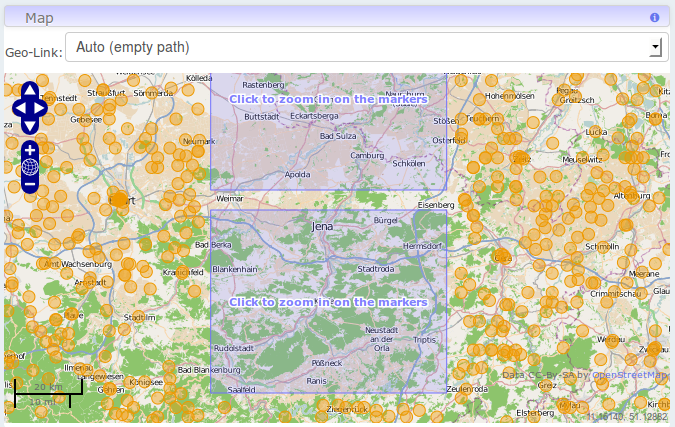
\includegraphics[width=0.5\textwidth]{images/facete-mii}
\caption{Display of Freebase instances in Germany.}
\label{fig:markers-freebase}
\end{figure}



\section{Related Work}
\label{sec:related-work}
The \emph{RelFinder} system~\cite{2009_relfinder} is capable of finding
property paths connecting a pair of \emph{resources}, whereas
Facete searches for paths between SPARQL \emph{concepts}.
Over the past decade, faceted search has become omnipresent, such as in
web shop and content management systems.
\emph{Apache Solr}\footnote{\url{http://lucene.apache.org/solr/}} is a popular system
that offers extensive faceted search features, however, it does not offer native
SPARQL support and thus requires pre-processing of RDF data.
\emph{Rhizomer}~\cite{2013_rhizomik} and the
\emph{Virtuoso faceted
browser}\footnote{\url{http://virtuoso.openlinksw.com/dataspace/dav/wiki/Main/VirtuosoFacetsWebService}}
support changing the focus from one set of resources to a related one
(known as pivoting). However, with these systems, the user actually navigates
between related list views of resources, whereas in Facete the user pins facets
as new columns to the table view.
%\emph{Sparallax}
%\footnote{\url{http://sparallax.deri.ie}}


%Pivoting (refocusing) 
% unconstrained and relational 

%Exhibit is often used for RDF data, it uses
%Facete offers this functionality directly on RDF.  


%While \todo{deri paper} investigate federated search based on SPARQL 1.1
%federation, we envision that SPARQL query federation engines, such as 
%FedEx and TopFed offer 

%Flint, Sparql-ed, YASGUI
%Ontowiki, (what about Calimachus?)


%Challenges:
%- Several geo vocabs - how to support them?
%- Large amount of spatial data

%- 
%Facete ful 
%\footnote{\url{http://geovocab.org}}
%\footnote{\url{}} georss
%\footnote{\url{http://www.opengeospatial.org/standards/geosparql}} geosparql
%\footnote{\url{http://docs.openlinksw.com/virtuoso/rdfsparqlgeospat.html}}


%\section{Implementation}
%github
%debian package
%Some limitations
%Computation of properties and their counts is affected by two dimensions:
%The current implementation of Facete attempts to retrieve all properties and
%their counts in a single query.
%Dimenions: Number of triples to scan - and number of distinct properties.
%This strategy works well for small datasets
%small datasets, sufficient constraints, few properties
%We are in the process af alleviating this limitation by 
%either small from the start, or thesufficiently constrained
%is based on the assumption that there is only a
%limited number of properties.
%DBpedia has \todo{count} properties, Freebase even.
%In the latter case, when excluding isbn numbers and users, still 100k remain.
%Initial experiments with DBpedia and Freebase
%showed that this assumpti


\section{Conclusions and Outlook}
\label{sec:conclusions}
In this demo we present \emph{Facete}, an advanced faceted browser
for SPARQL accessible data with geo-spatial capabilities.
We demonstrate Facete's potential based on a sophisticated use case
which requires retrieval of information from a set of
indirectly related resources. Users are empowered to create customizable a tabular data views showing attributes they are interested in. 
Based on related geometric information, these data are also shown on a map.
% and can browse these data on
%the map.
Facete's three key concepts are:
(1) The generic faceted filtering engine,
that supports showing and filtering by nested facets, (2) the property path
detection, which efficiently detects how resources can be shown on the map based
on indirectly related spatial information, and (3) how the system offers an
interactive map display even in the face of large amounts of geometric
information.

There are a number of directions for future work: One is adding support for aggregation
functions. Another logical step is to define more advanced views than
the current table and map.
Users should then be empowered to connect such views to their created data
table. For instance, once a user has defined a table which lists for each city
or country the total amount of money given to partners
located in it, then based on this information a heat map view could be rendered.
Our vision is, for the creation of visualizations from Linked
Data to become as simple as in spreadsheet applications,
where advanced chart and map visualizations can be created with a few clicks.
%Unlike conventional spreadsheets, however, the use of
%(quasi-)standard vocabularies could serve a convention over configuration
% approach

%Furthe definition of multiple data tables that may be related
%to each other. 



%A quad tree is a space partition tree where each node is partitioned into
% 4 children. Objects cannot 'sink' in a child node if they overlap a
% partition border. Loose quad trees allow child nodes to overlap to some
% extent, thus allowing objects overlapping the root nodes border
% potentially deeper in the tree.
 
%\section{Demonstration}


% We can add this for the camera-ready submission:
%\section{Acknowledgment}
%This work was supported by grants from the EU's 7th Framework Programme
%provided for the projects LOD2 (GA no. 257943) and GeoKnow (GA no. 611845).

%\bibliographystyle{abbrv}
%\bibliography{bibliography,../../bib/aksw}

%\end{document}


